\newpage
\appendix
\chapter{Experiment Code}
\begin{lstlisting}[language=Python, caption= Training code, label=ls:train_code]
import pdb
import argparse
from typing import List, Dict
from types import SimpleNamespace
import multiprocessing as mp
import time

import numpy as np
import scipy as sp
import torch
import torch.nn as nn
import torch.nn.functional as F
import torch.optim as optim
from sklearn.metrics import f1_score
from sklearn.linear_model import LinearRegression
from torchviz import make_dot

from module import GCN, GCNLinear
from load_data import load_random_block
from sampler import full_sampler, ladies_sampler
from utils import adj_to_lap_matrix, row_normalize, sparse_mx_to_torch_sparse_tensor, sparse_fill


#np.seterr(all="raise")

def random_sampling_train(args: SimpleNamespace, model: SimpleNamespace, data: SimpleNamespace) -> SimpleNamespace:
  if args.batch_size <= 0 or args.batch_size >= len(data.train_nodes):
    batch_nodes = data.train_nodes
  else:
    batch_nodes = np.random.choice(data.train_nodes, size= args.batch_size, replace= True)
  sample = model.sampler(
    batch_nodes= batch_nodes,
    samp_num_list= [len(batch_nodes) for _ in range(args.num_layers)],
    num_nodes= data.num_nodes,
    lap_matrix= data.lap_matrix,
    lap2_matrix= data.lap2_matrix,
    num_layers= args.num_layers,
  )
  return sample

def sampling_valid(args: SimpleNamespace, model: SimpleNamespace, data: SimpleNamespace) -> SimpleNamespace:
  sample = full_sampler(
    #batch_nodes= data.valid_nodes,
    batch_nodes= np.arange(data.num_nodes),
    samp_num_list= None,
    num_nodes= data.num_nodes,
    lap_matrix= data.lap_matrix,
    lap2_matrix= None,
    num_layers= args.num_layers,
  )
  return sample



if __name__ == "__main__":
  # load args
  parser = argparse.ArgumentParser(description='Training GCN')
  parser.add_argument('--hidden_features', type=int, default=64,
                      help='hidden layer embedding dimension')
  parser.add_argument('--num_epochs', type=int, default= 10,
                      help='Number of epochs')
  parser.add_argument('--batch_size', type=int, default=64,
                      help='batch_size: number of sampled nodes at output layer')
  parser.add_argument('--num_layers', type=int, default=5,
                      help='Number of GCN layers')
  parser.add_argument('--sampling_method', type=str, default='full',
                      help='sampling algorithms: full/ladies')
  parser.add_argument('--cuda', type=int, default=-1,
                      help='GPU ID, (-1) for CPU')
  parser.add_argument('--dropout', type=float, default= 0.5,
                    help='dropout probability')
  parser.add_argument('--learning_rate', type=float, default= 1e-3,
                    help='learning rate')
  parser.add_argument('--num_nodes', type=int, default=100,
                      help='number of network nodes in random block model')

  args = parser.parse_args()
  print(args)
  # set up device
  if args.cuda != -1:
    device = torch.device("cuda:" + str(args.cuda))
  else:
    device = torch.device("cpu")
  # load data
  all = args.num_nodes
  half = int(all/2)
  p1 = np.log(all) / all
  p2 = p1 / all
  data = load_random_block(
    [half, all-half],
    [[p1, p2], [p2, p1]],
  )
  data.num_nodes = data.features.shape[0]
  data.in_features = data.features.shape[1]
  data.out_features = len(np.unique(data.labels))
  data.lap_matrix = row_normalize(adj_to_lap_matrix(data.adj_matrix))
  data.lap2_matrix = data.lap_matrix.multiply(data.lap_matrix)

  if args.sampling_method == "full":
    args.batch_size = len(data.train_nodes)
  # create pool
  pool = mp.Pool(processes= 1)
  # create model
  model: SimpleNamespace = SimpleNamespace()
  model.sampler = full_sampler
  if args.sampling_method == "ladies":
    model.sampler = ladies_sampler
  model.module = GCNLinear(
    encoder= GCN(
      in_features= data.in_features,
      hidden_features= args.hidden_features,
      out_features= args.hidden_features,
      num_layers= args.num_layers,
      dropout= args.dropout
    ),
    in_features= args.hidden_features,
    out_features= data.out_features,
    dropout= args.dropout,
  )


  model.module.to(device)
  optimizer = optim.Adam(filter(lambda p: p.requires_grad, model.module.parameters()), lr=args.learning_rate)
  criterion = nn.CrossEntropyLoss()
  times = []
  losses = []
  f1s = []
  next_sample_async = None
  sample = None

  #START TRAINING
  start = time.time()
  try:
    for epoch in range(args.num_epochs):
      # train
      model.module.train() # train mode
      print(f"Epoch {epoch}: ", flush= True)
      num_iterations = int(data.num_nodes / args.batch_size)
      for iter in range(num_iterations):
        print(f"\tIteration {iter}: ", end= "", flush= True)
        if next_sample_async is None:
          sample = random_sampling_train(args, model, data)
        else:
          sample = next_sample_async.get()
        next_sample_async = pool.apply_async(random_sampling_train, args= (args, model, data))
        optimizer.zero_grad()
        
        output = model.module(
          x= sparse_mx_to_torch_sparse_tensor(sparse_fill(shape= data.features.shape, mx= data.features[sample.input_nodes], row= sample.input_nodes)),
          adjs= list(map(lambda adj: sparse_mx_to_torch_sparse_tensor(adj).to(device), sample.adjs)),
        )

        loss = criterion(
          output[sample.output_nodes],
          torch.from_numpy(data.labels[sample.output_nodes]).long(),
        )
        loss.backward()
        torch.nn.utils.clip_grad_norm_(model.module.parameters(), 0.2)
        optimizer.step()


        #if epoch == 0 and iter == 0:
        #  dot = make_dot(loss.mean(), params= dict(model.module.named_parameters()))
        #  dot.render("test.gv", view= True)

        loss = loss.detach().cpu()
        print(f"Loss {loss}", flush= True)
      # eval
      model.module.eval() # eval mode
      sample = sampling_valid(args, model, data)
      output = model.module(
        x= sparse_mx_to_torch_sparse_tensor(data.features[sample.input_nodes]),
        adjs= list(map(lambda adj: sparse_mx_to_torch_sparse_tensor(adj).to(device), sample.adjs)),
      )
      loss = criterion(
        output[sample.output_nodes],
        torch.from_numpy(data.labels[sample.output_nodes]).long(),
      )
      
      output = output.detach().cpu()
      loss = loss.detach().cpu()
      f1 = f1_score(
        output[sample.output_nodes].argmax(dim=1),
        data.labels[sample.output_nodes],
        average= "micro",
      )
      times.append(time.time() - start)
      losses.append(loss)
      f1s.append(f1)

      epochs = np.arange(len(times)).reshape(-1, 1)
      reg = LinearRegression().fit(epochs, times)
      eta = reg.predict(np.array(args.num_epochs - 1).reshape(-1, 1))[0]
      
      print(f"Epoch {epoch}: Loss {loss} F1 {f1} ETA {eta - time.time() + start}s", flush= True)

  except KeyboardInterrupt:
    pass
  print(f"Elapsed Time: {time.time() - start}")

  import matplotlib.pyplot as plt
  fig, axs = plt.subplots(nrows= 2, ncols= 2, constrained_layout=True)
  fig.suptitle(f"Sampling method: {args.sampling_method}, Number of nodes {args.num_nodes}")
  
  axs[0][0].plot(np.arange(len(times)), losses)
  axs[0][0].set_xlabel("Epoch")
  axs[0][0].set_ylabel("Loss")

  axs[0][1].plot(times, losses)
  axs[0][1].set_xlabel("Time")
  axs[0][1].set_ylabel("Loss")


  axs[1][0].plot(np.arange(len(times)), f1s)
  axs[1][0].set_xlabel("Epoch")
  axs[1][0].set_ylabel("F1")

  axs[1][1].plot(times, f1s)
  axs[1][1].set_xlabel("Time")
  axs[1][1].set_ylabel("F1")

  plt.show()
  
\end{lstlisting}


\chapter{Experiment Plots}
\label{experiment_plots}

\begin{figure}[H]
    \centering
    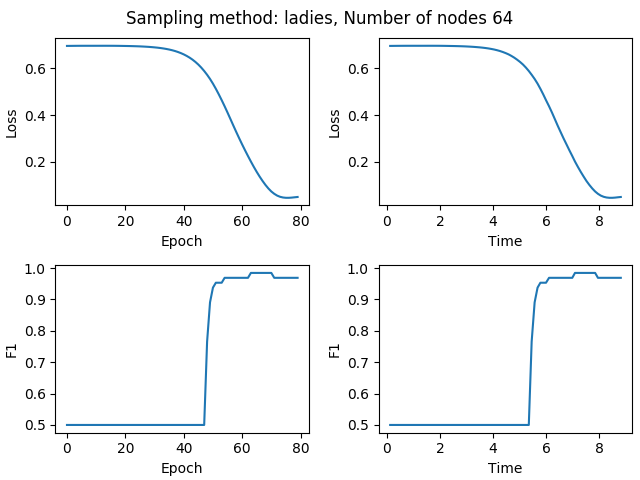
\includegraphics[scale=0.8, ]{assets/plots/ladies_64.png}
    \caption{Ladies with 64 nodes} 
\end{figure}

\begin{figure}[H]
    \centering
    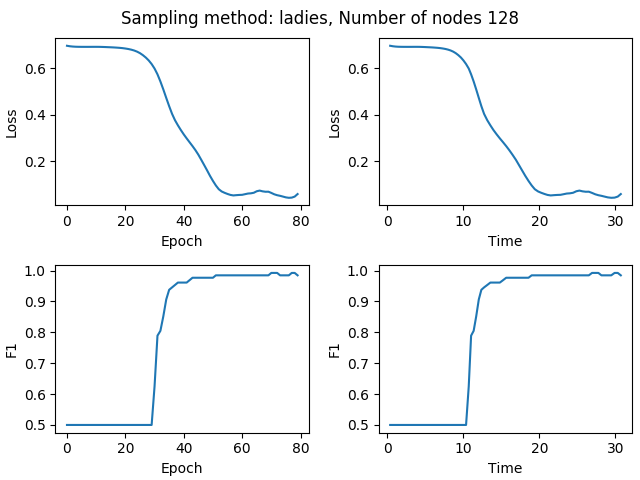
\includegraphics[scale=0.8, ]{assets/plots/ladies_128.png}
    \caption{Ladies with 128 nodes} 
\end{figure}

\begin{figure}[H]
    \centering
    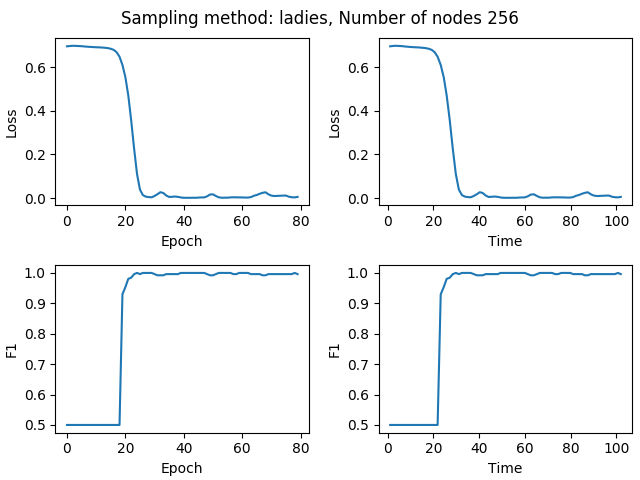
\includegraphics[scale=0.8, ]{assets/plots/ladies_256.png}
    \caption{Ladies with 256 nodes} 
\end{figure}

\begin{figure}[H]
    \centering
    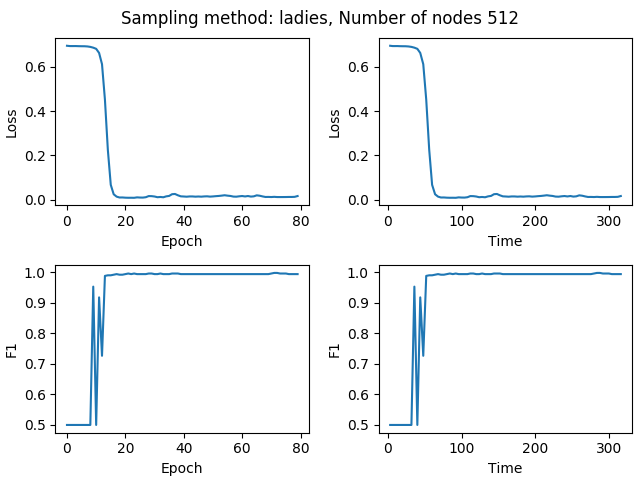
\includegraphics[scale=0.8, ]{assets/plots/ladies_512.png}
    \caption{Ladies with 512 nodes}
\end{figure}

\begin{figure}[H]
    \centering
    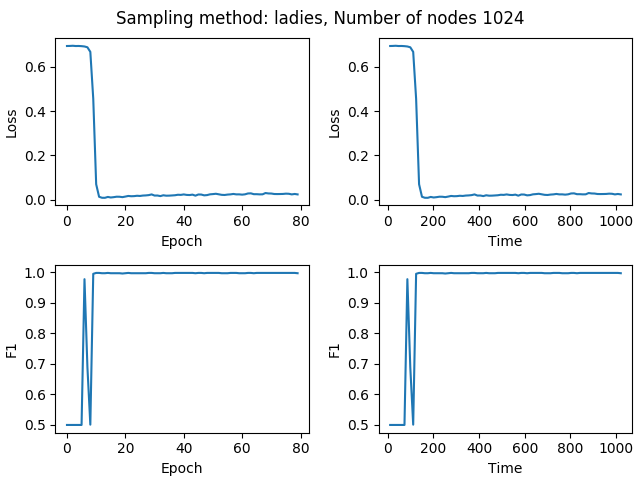
\includegraphics[scale=0.8, ]{assets/plots/ladies_1024.png}
    \caption{Ladies with 1024 nodes}
\end{figure}

\begin{figure}[H]
    \centering
    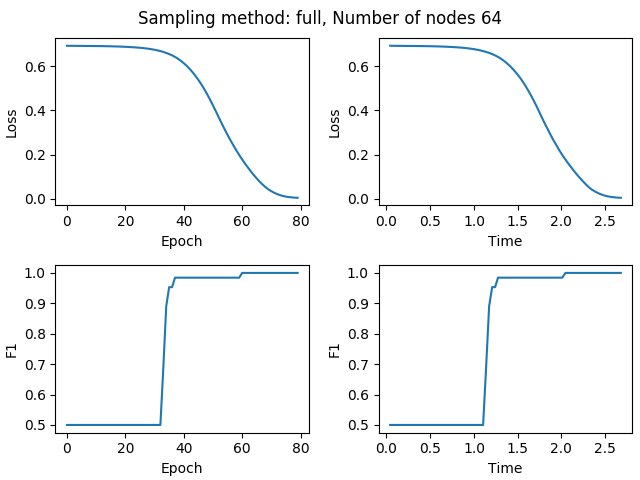
\includegraphics[scale=0.8, ]{assets/plots/full_64.png}
    \caption{Full GCN with 64 nodes}
\end{figure}

\begin{figure}[H]
    \centering
    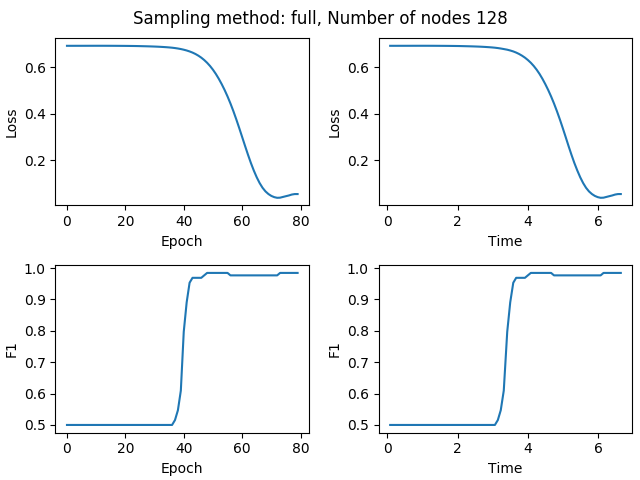
\includegraphics[scale=0.8, ]{assets/plots/full_128.png}
    \caption{Full with 128 nodes}
\end{figure}

\begin{figure}[H]
    \centering
    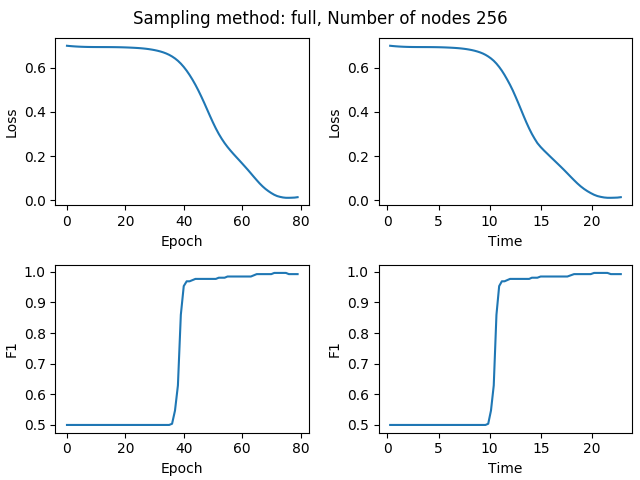
\includegraphics[scale=0.8, ]{assets/plots/full_256.png}
    \caption{Full GCN with 256 nodes}
\end{figure}

\begin{figure}[H]
    \centering
    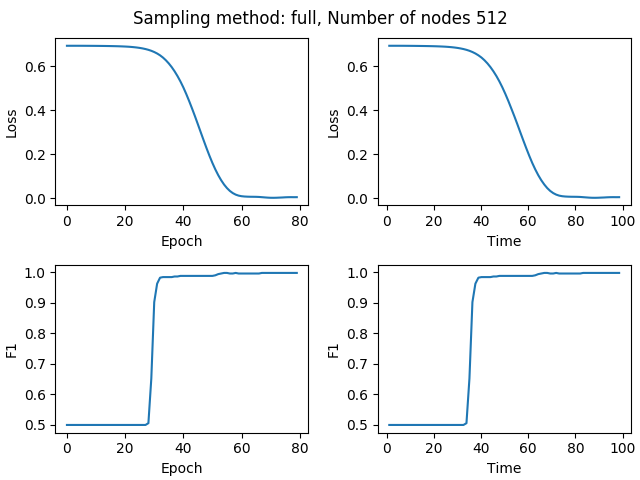
\includegraphics[scale=0.8, ]{assets/plots/full_512.png}
    \caption{Full GCN with 512 nodes}
\end{figure}

\begin{figure}[H]
    \centering
    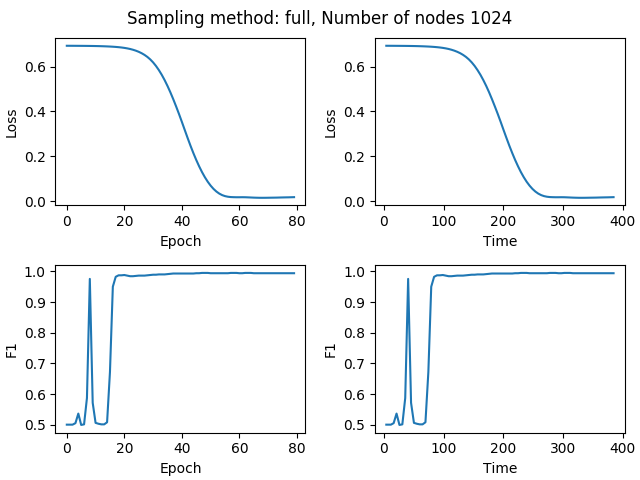
\includegraphics[scale=0.8, ]{assets/plots/full_1024.png}
    \caption{Full GCN with 1024 nodes}
\end{figure}